% !TeX spellcheck = en_US
\documentclass{extarticle}

\usepackage{graphicx}

\begin{document}
	\section{Part 3}
	\begin{figure}[ht!]
		\centering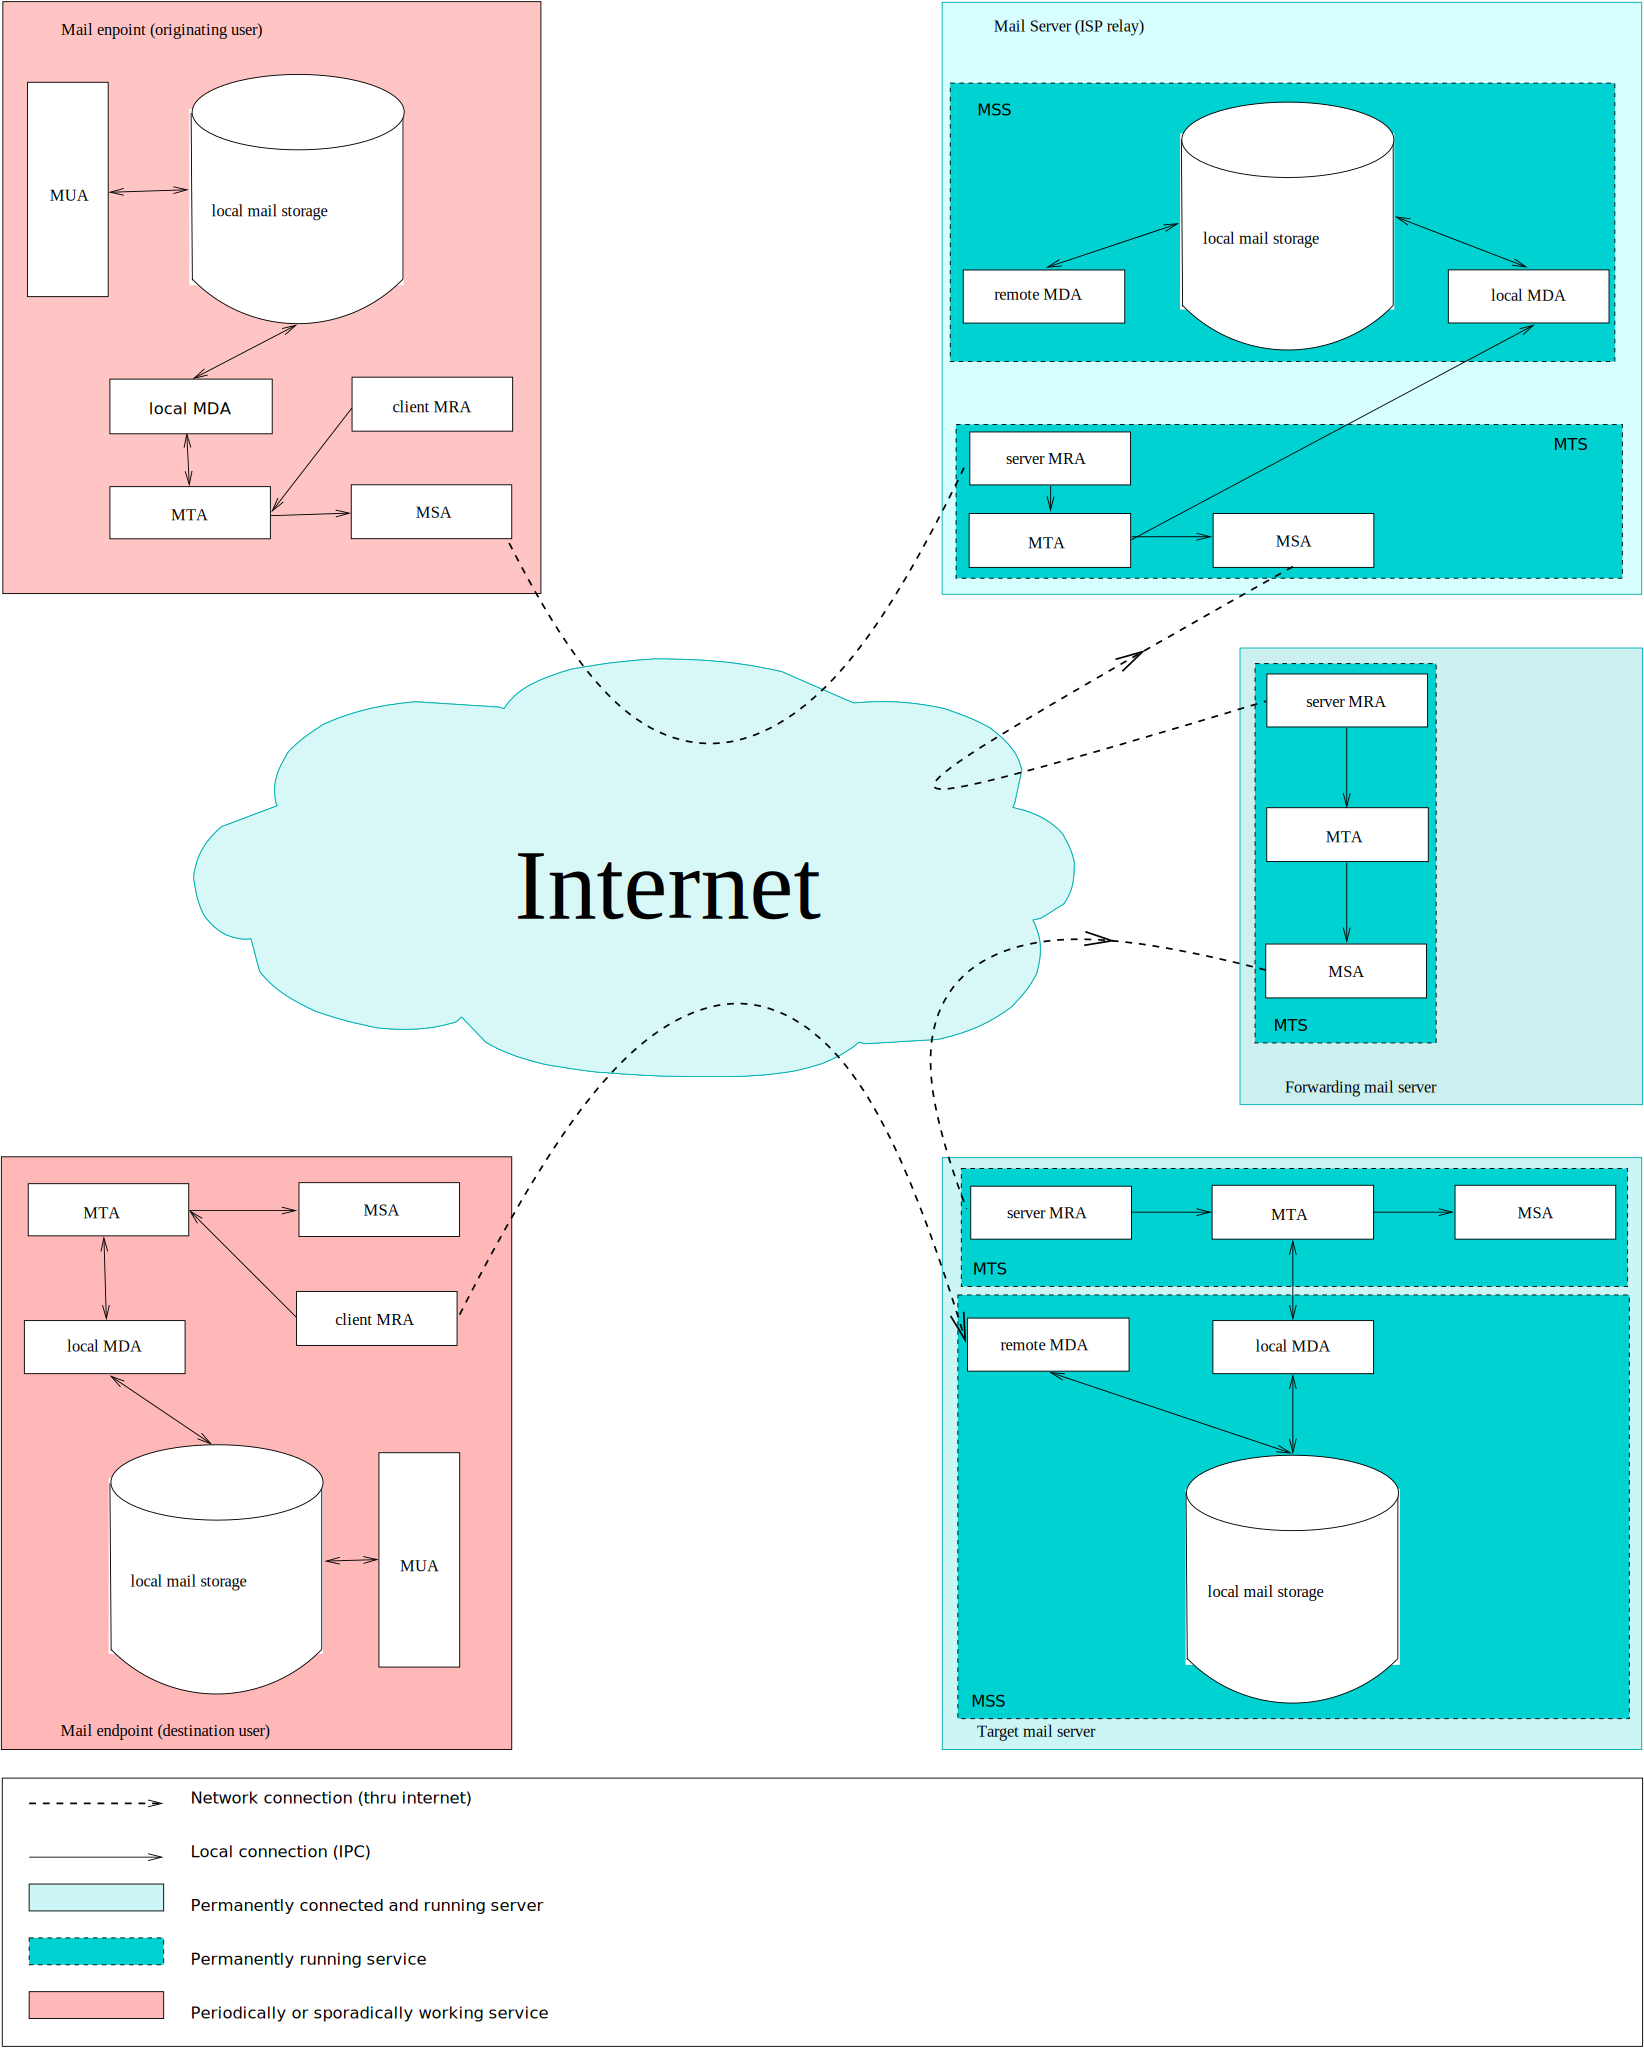
\includegraphics[width=\columnwidth]{inc/MailAgents1.pdf}
		\caption{Mail Agents}
		\label{fig:MailAgents}
	\end{figure}
	This Figure is at the beginning of part 3. It shows the relevant services of a mail router in a modified way.
	
	\section{Part 4}
	
	\begin{figure}[ht]\centering
		\includegraphics[width=0.8\columnwidth]{inc/addRedundancyOp}
		\caption{Outline of the addRedundancy operation}
		\label{fig:addRedundancyOperation}
	\end{figure}
	This figure describes a core operation. It first takes an input vector, pads and splits it into a series of blocks, then applies an operation on it, and then executes an unpadded, symmetric encryption operation. This is one of the operations which is part in one of the subsequent graphics.
	
	
\end{document}